\chapter{}

\epigraph{"If 10 years from now, when you are doing something quick and dirty, you suddenly visualize that I am looking over your shoulders and say to yourself: 'Dijkstra would not have liked this', well that would be enough immortality for me."}{\textit{Edsger W. Dijkstra}}

\section*{The LEGv8 simulators landscape}

The current landscape of publicly available LEGv8 simulators can be divided into two categories: simulators that aim to reproduce the logical design presented in the textbook in chapter ?, and the simulators providing a high level simulation of the instruction set as defined in the book.
The survey was performed on GitHub using ``LEGv8'' and ``simulator'' as keywords and only those in a reasonably working state (as per the author) have been considered.

\subsection*{Software simulators}

\begin{table}[H]
	\centering
	\resizebox{\columnwidth}{40}{\small \begin{tabular}{|c|c|c|c|c|c|c|}
		\hline
		\textbf{Repository} & \textbf{Language} & \textbf{Integer Support} & \textbf{Pipelined} & \textbf{Registers view} & \textbf{Stack view} & \textbf{Floating Point Support} \\
		\hline
		\url{https://github.com/lcpckp/leg-cpu-sim} & Java & Partial & No & Yes & Yes & No \\
		\hline
		\url{https://github.com/chrwoods/legv8-emul} & C/C++ & Partial & Yes & Yes & Yes & No \\
		\hline
		\url{https://github.com/mtalyat/LEGv8Day} & C\# & Partial & No & Yes & Yes & No \\
		\hline
		\url{https://github.com/eaxworthy/LegV8Interpreter} & Python & Partial & No & Yes & Yes & No\\
		\hline
		\url{https://github.com/AdinAck/LEGv8-Simulator} & Swift & Partial & No & Yes & Yes & No \\
		\hline
		\url{https://github.com/anvitha305/legv8sim} & Python & Partial & No & Yes & Yes & Double precision only \\
		\hline
		\url{https://github.com/dangbandy/LegV8-Simulator} & C++ & Partial & No & Yes & Yes & No\\
		\hline
		\url{https://github.com/schang412/LEGv8-PyEmu} & Python & Partial & No & No & No & No\\
		\hline
		\url{https://github.com/GeorgePerreault/LEGV8_Interpreter} & Python & Partial & No & Yes & Yes & No\\
		\hline
	\end{tabular}}
	\caption{The surveyed software simulators}
\end{table}

They utilize high level languages such as C++, Python, Swift, TypeScript and Java. Some of them offer a graphical interface, pipelined execution and none of the implement the LEGv8 ISA in its entirety.



\subsection*{Hardware simulators}

\begin{table}[H]
	\centering
	\resizebox{\columnwidth}{45}{\small \begin{tabular}{|c|c|c|c|c|c|c|}
		\hline
		\textbf{Repository} & \textbf{Language} & \textbf{Integer Support} & \textbf{Pipelined} & \textbf{Floating Point Support} \\
		\hline
		\url{https://github.com/nxbyte/ARM-LEGv8} & Verilog & Partial & Yes & No \\
		\hline
		\url{https://github.com/phillbush/legv8} & Verilog & Partial & Yes & No \\
		\hline
		\url{https://github.com/ronitrex/ARMLEG} & Verilog & Partial & Yes & No \\
		\hline
		\url{https://github.com/mattco98/LEGv8-Processor} & Verilog & Partial & Yes & Partial \\
		\hline
		\url{https://github.com/amaurilopez90/LEGv8-CPU} & Verilog & Partial & Yes & No \\
		\hline
		\url{https://github.com/miguelangelo78/LEGv8-ISA} & Verilog & Partial & Yes & No \\
		\hline
		\url{https://github.com/brianworts/LEGv8_SingleCycle_Processor} & Verilog & Partial & Yes & No \\
		\hline
		\url{https://github.com/egflo/LEGv8} & Verilog & Partial & Yes & No \\
		\hline
		\url{https://github.com/ad153153/LegV8} & Verilog & Partial & Yes & No \\
		\hline
	\end{tabular}}
	\caption{The surveyed hardware simulators}
\end{table}

They use mostly Verilog as their hardware description language and implement an incomplete subset of the LEGv8 ISA. Some of them follow closely the design of the textbook while others expand upon it adding more executable instructions. None of them offer a graphical interface nor implement the ISA in its entirety.
\\

It is clear from this brief survey that the LEGv8 simulators space lacks any desirable candidates for code execution and inspection, as the software simulators are incomplete and platform-dependant, and the hardware ones lack interactivity and comprehensive visual output capabilities.

\section*{ARM's LEGv8 simulator}

This is the simulator officially provided by ARM Education and is the subject of this thesis' work. It is written in Java 8 and uses Google's GWT framework to transpile the code into native JavaScript to allow the simulator to be executed inside a web browser as a normal web application. It provides a comprehensive user interface displaying an interactive text editor (provided by AceGWT) to input LEGv8 code and to display errors, and a visualization of the state of the \emph{X} registers.
When selecting the single-cycle execution mode, a visualizaton of the logical scheme of the LEGv8 ISA is presented and for each step of the execution various components change color to indicate the current stage of the pipeline. For the pipelined execution mode, the visualization is slightly modified to include pipeline-specific information such as pipeline registers, the hazard detection unit and the forwarding unit. An additional textual representation of the pipeline is provided to see the stage occupied by each instruction at any given moment.

\begin{figure}[H]
	\centering
	\subfigure[Single cycle]{
		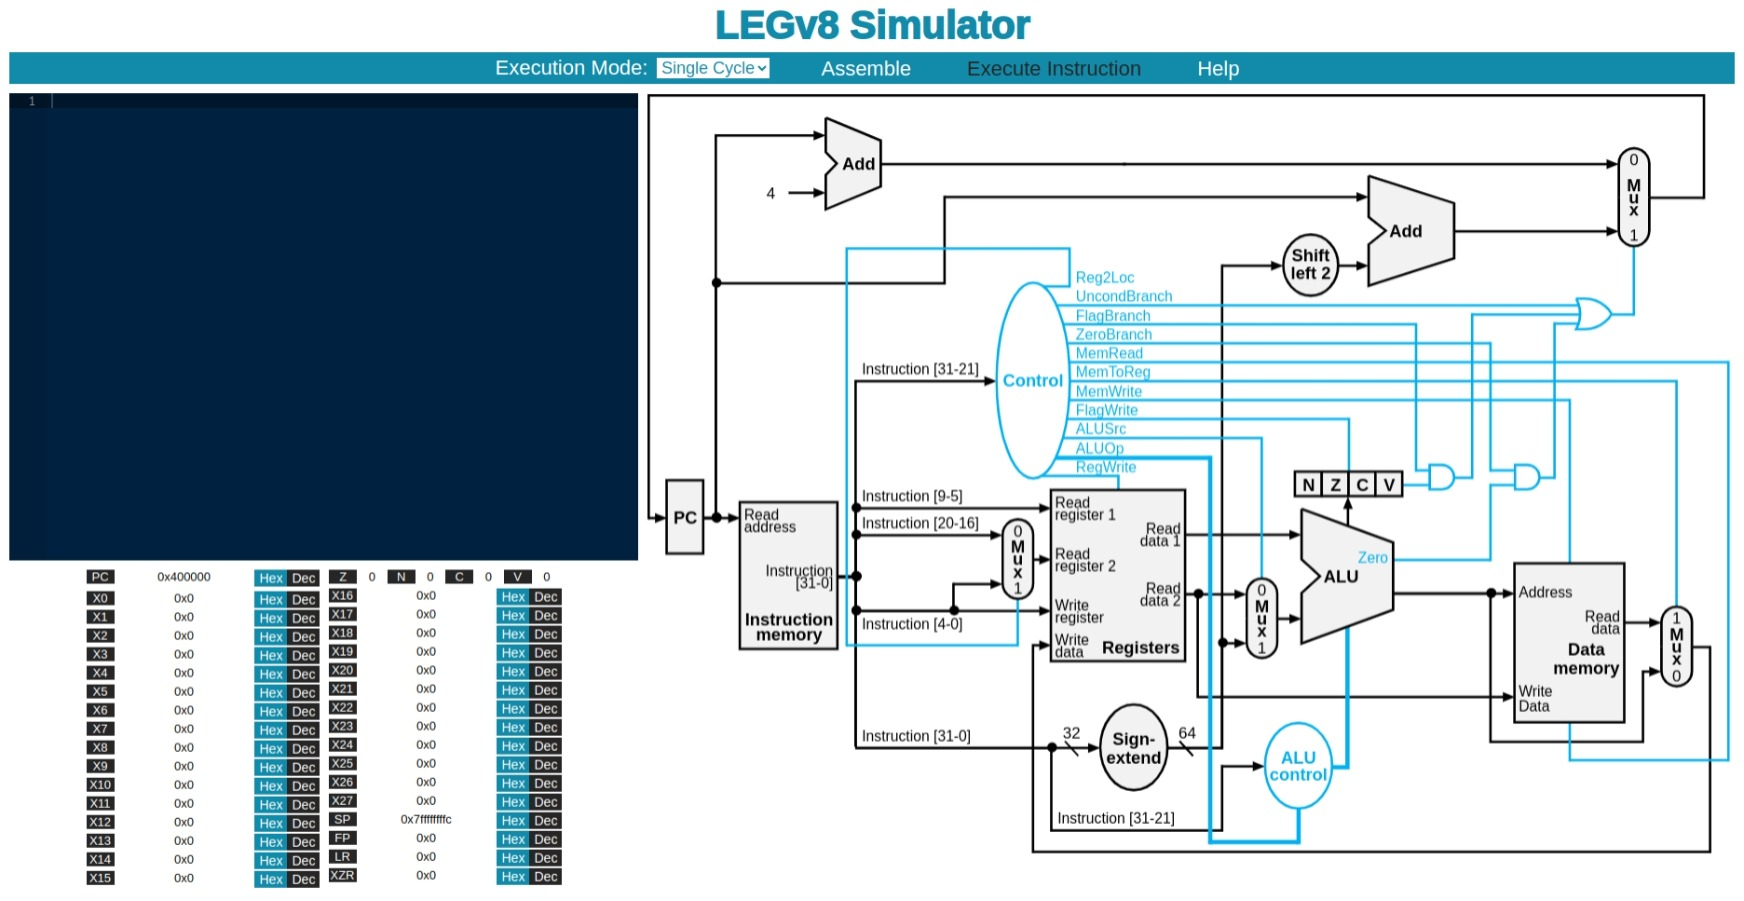
\includegraphics[width=.85\textwidth]{img/old_single_cycle.jpeg}
	}
	
	\subfigure[Pipeline]{
		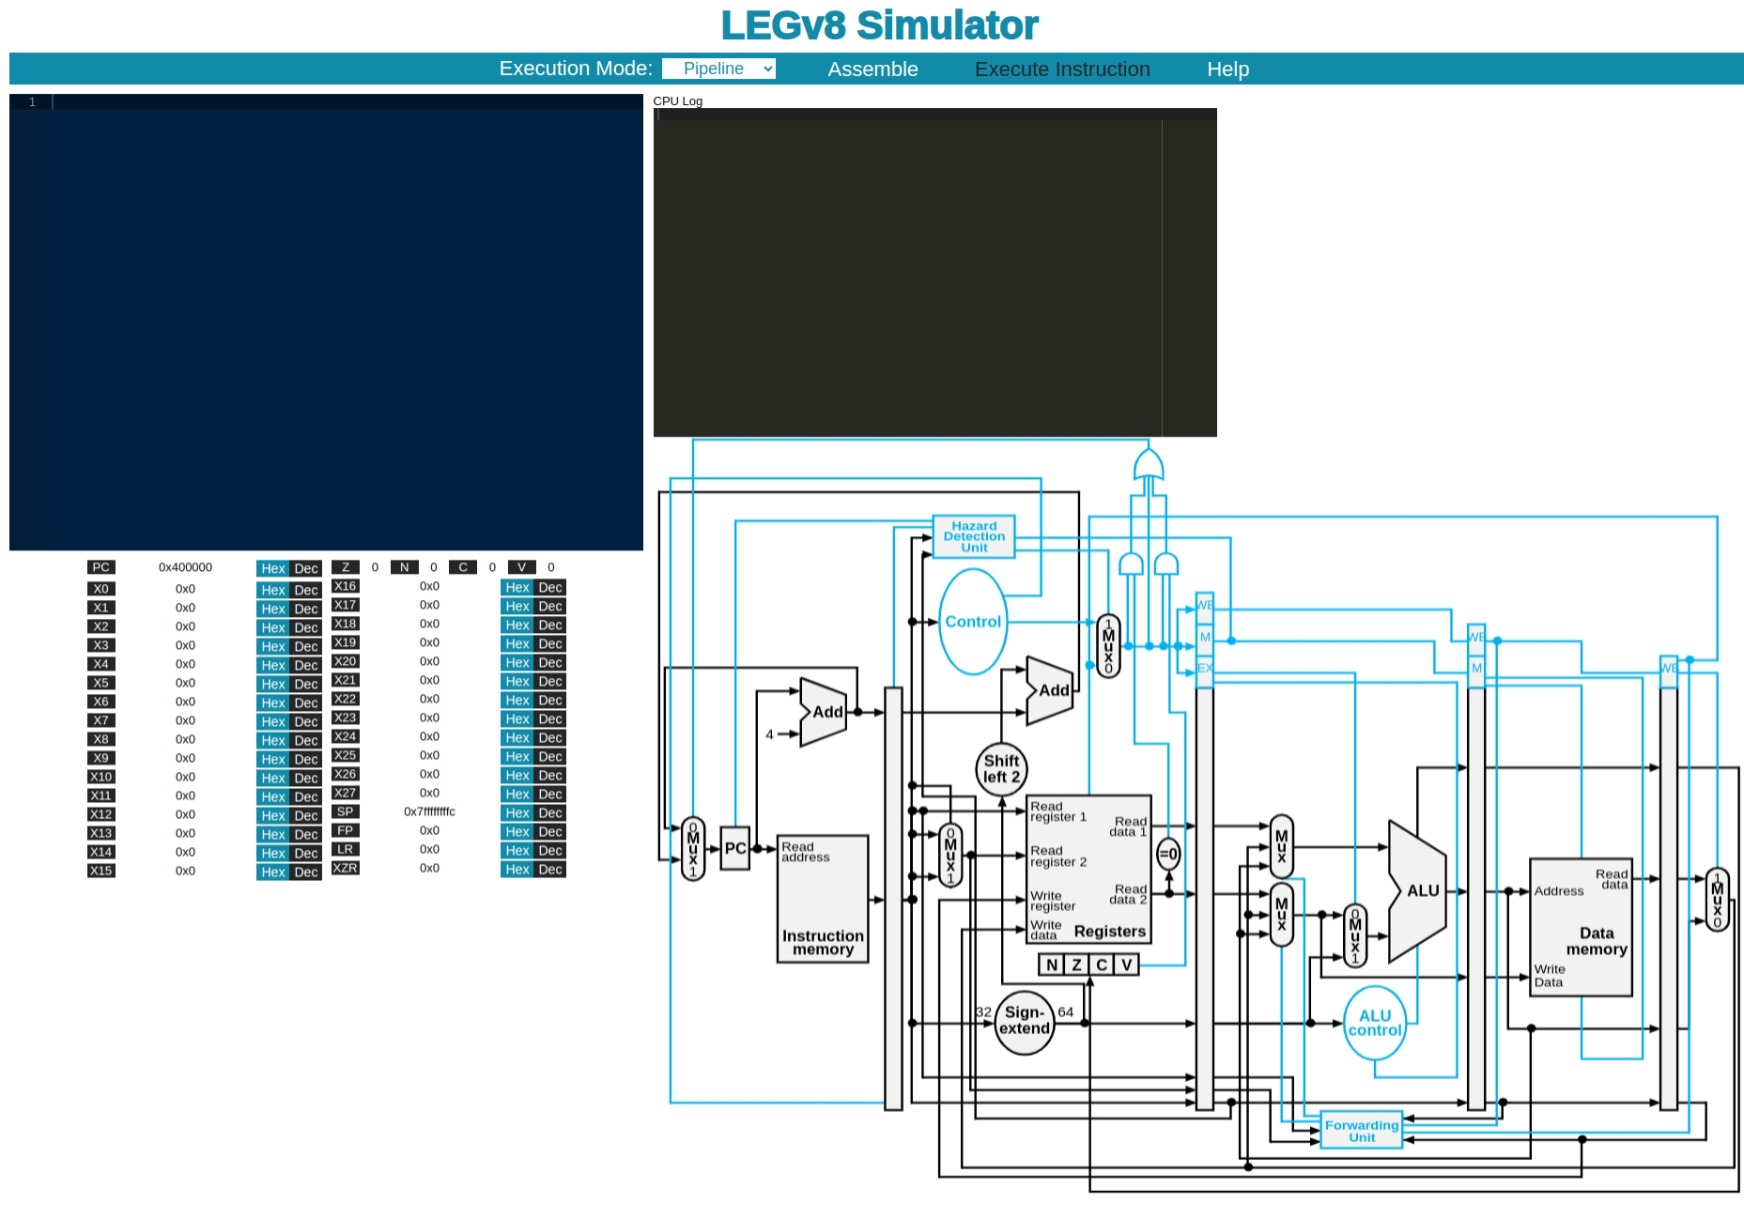
\includegraphics[width=.85\textwidth]{img/old_pipeline.jpeg}
	}
	\caption{The simulator's main page with the two different execution modes}
\end{figure}

\subsection*{Features}

This simulator presents many favorable characteristics:

\begin{itemize}[label=\textendash]
	\item Written in Java (platform agnostic, extensible)
	\item Compiled as a web application (platform agnostic and easily deployable)
	\item Embedded text editor to input code with, and error display
	\item Clear and rich visualization of the \emph{X} and flag registers and the datapath of the CPU
	\item Almost all of the integer arithmetic is already implemented
	\item All types of integer \emph{LOAD} and \emph{STORE} instructions are already implemented, including \emph{STXUR} and \emph{LDXUR}
	\item Officially distributed by ARM Education (biggest support and discoverability)
\end{itemize}


\subsection*{Problems}

Unfortunately many problems present themselves when trying to run or develop the simulator:

\begin{itemize}[label=\textendash]
	\item Absence of any documentation on how to build the project and design choices behind it
	\item Executable version distributed in automatically-generated web page form
	\item Pipeline execution is incomplete
	\item The mechanism for calling subroutines is broken and results in infinite loops, making it impossible to delegate code to other functions
	\item The mechanism for performing comparisons is broken and results in the wrong branches being taken, making it impossible to perform conditional operations and loops
	\item The project is heavily dependent on the Eclipse Java IDE with an old GWT plugin to perform the build process
	\item The project depends on the outdated and barely supported GWT library to deploy the simulator as a web application. This restricts the developers from using newer Java features or better web frameworks.
\end{itemize}


I present below a demonstration of the bugs regarding the subroutine calls and number comparisons:

\begin{figure}[H]
	\centering
	\subfigure[BL instruction writes the incorrect address to the return register (LR)]{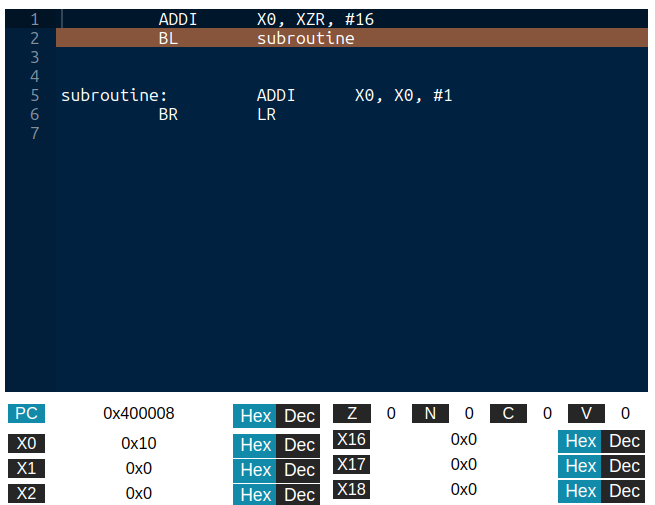
\includegraphics[width=.45\textwidth]{img/br_bug_1.png}}
	\subfigure[Jumps to the subroutine and increments X0]{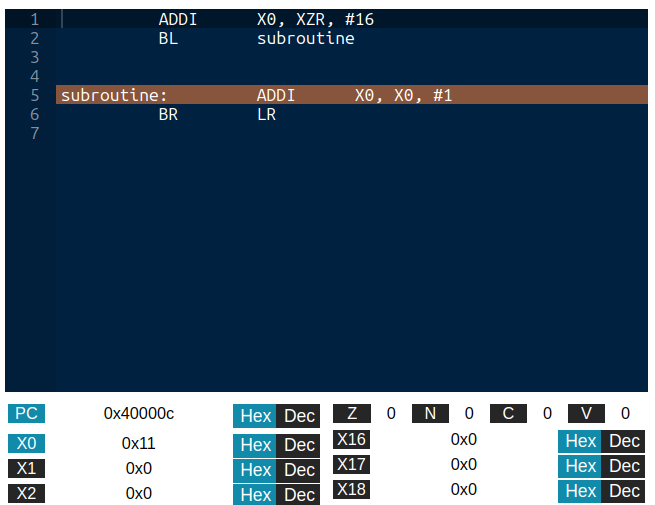
\includegraphics[width=.45\textwidth]{img/br_bug_2.png}}
	\subfigure[Reads wrong address from LR]{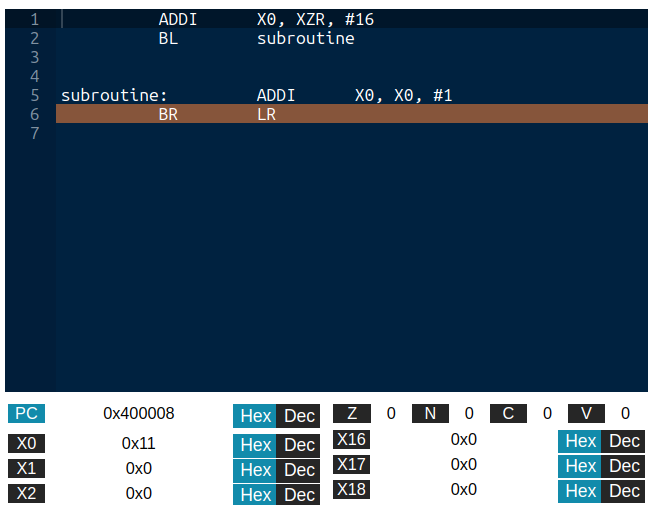
\includegraphics[width=.45\textwidth]{img/br_bug_3.png}}
	\subfigure[Returns to the start of the subroutine instead of the main program]{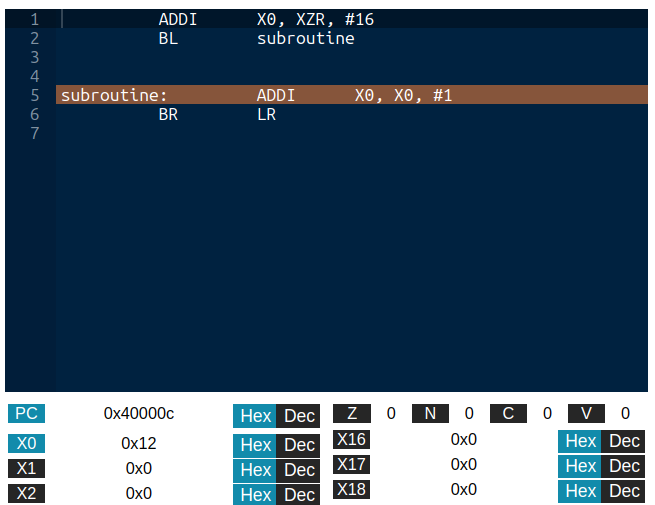
\includegraphics[width=.45\textwidth]{img/br_bug_4.png}}
	\caption{Branch returns to the wrong instruction, making it execute the branch in a loop}
\end{figure}

\begin{figure}[H]
	\centering
	\subfigure[X0 < X1]{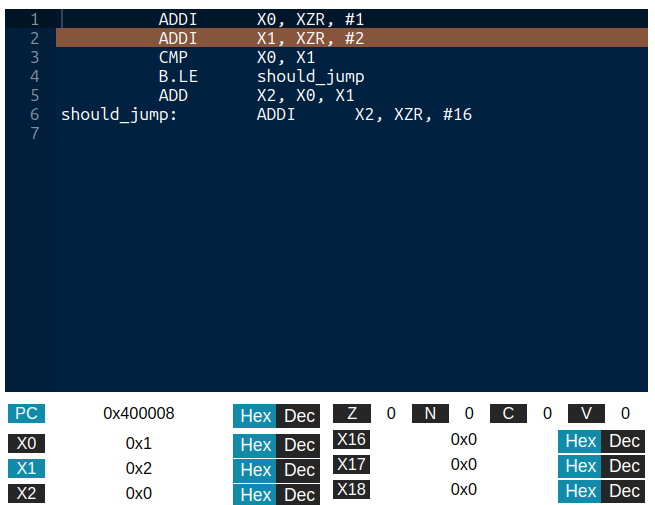
\includegraphics[width=.45\textwidth]{img/cmp_bug_1.png}}
	\subfigure[Comparison sets the flags incorrectly]{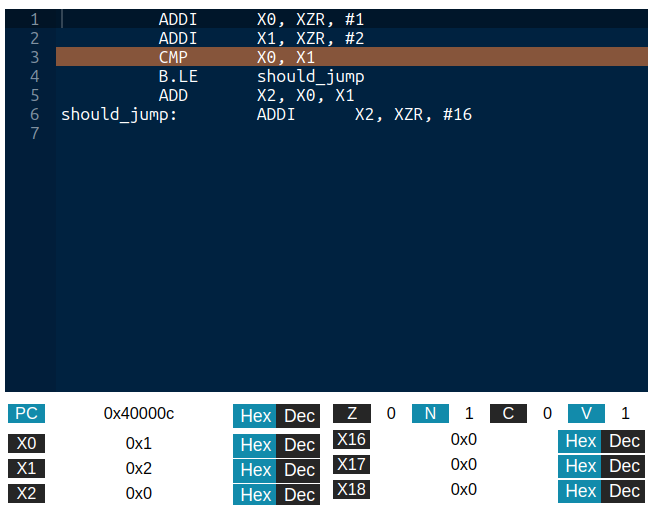
\includegraphics[width=.45\textwidth]{img/cmp_bug_2.png}}
	\subfigure[Branch gets ignored]{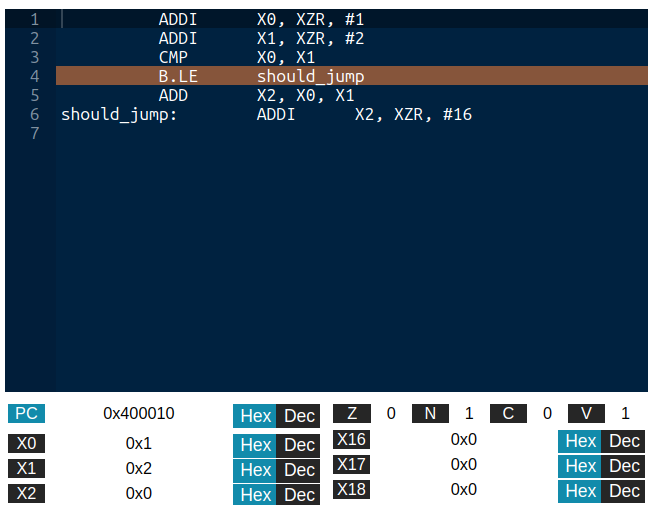
\includegraphics[width=.45\textwidth]{img/cmp_bug_3.png}}
	\subfigure[Wrong instruction executed]{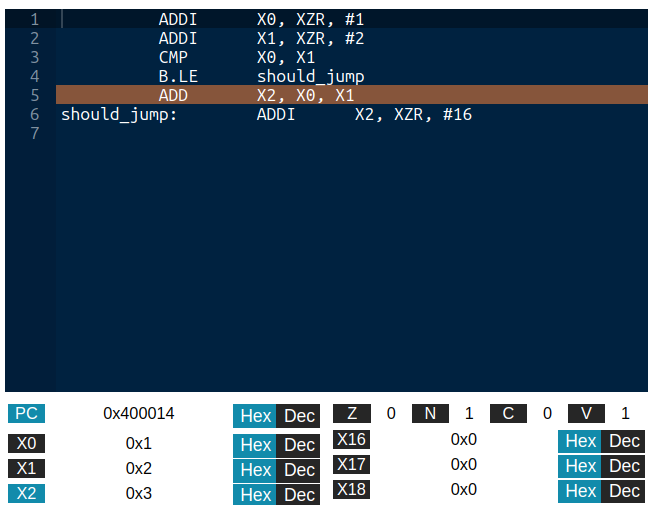
\includegraphics[width=.45\textwidth]{img/cmp_bug_4.png}}
	\caption{Comparisons do not set the correct flags and thus fail}
\end{figure}

\subsection*{Motivations}

For these reasons, this simulator was chosen as the subject of my thesis:

\begin{itemize}[label=\textendash]
	\item Maximize the impact of my work by fixing and improving the most popular simulator available
	\item Provide the first complete implementation of the LEGv8 instruction set
	\item Allow the Digital Systems Architecture course at UniTS and other courses in general to have a working LEGv8 simulator for more effective teaching
	\item Opportunity to work on a real Java code base
\end{itemize}